\section{Experiment}
    \subsection{Data Preprocessing}
        \begin{figure}[tbh]
            \centering
            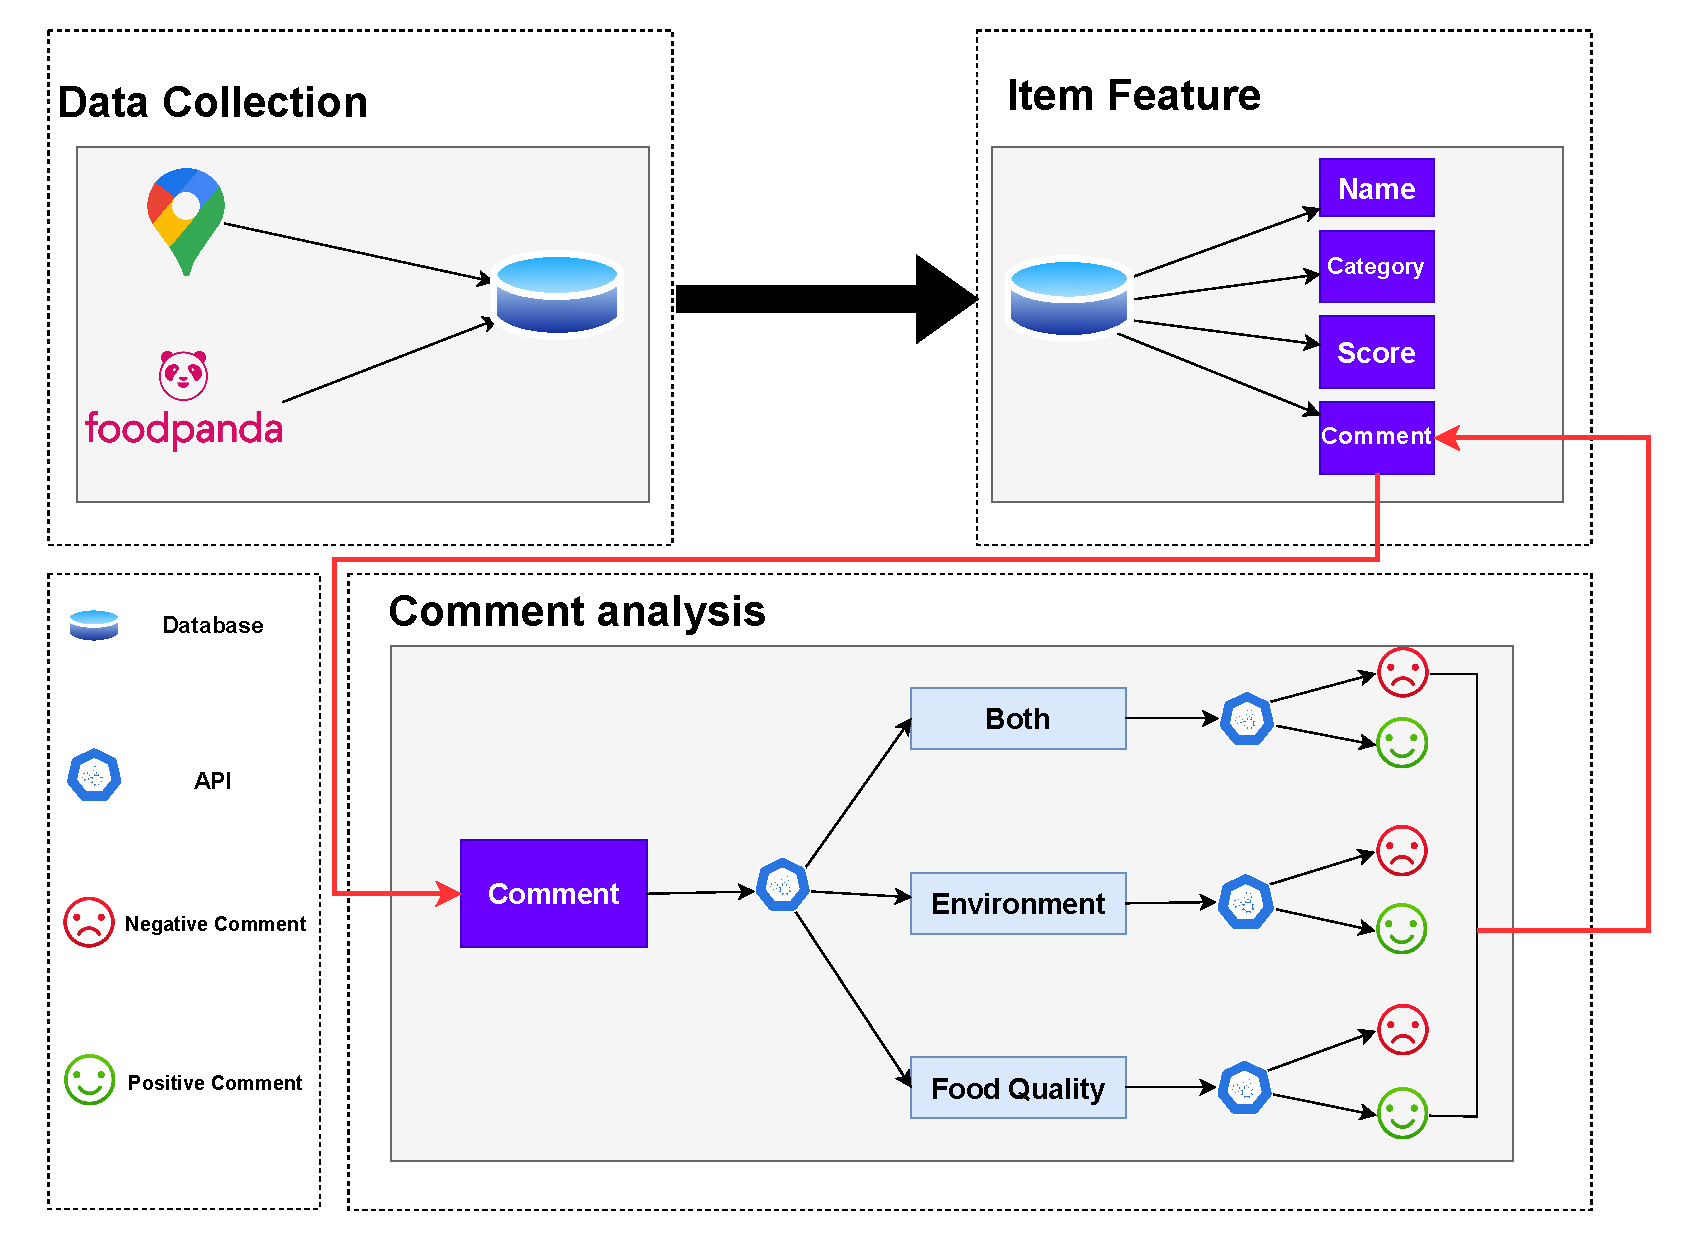
\includegraphics[width=0.5\textwidth]{img/preprocess.pdf}
            \caption{資料前處理架構圖}
            \label{fig-preprocess}
        \end{figure}
        本研究的資料前處理架構如\xfig{fig-preprocess}所示,透過爬蟲技術從 Foodpanda 與 Google Maps 收集餐廳相關資料。每間餐廳的資料包含餐廳名稱、類型、評分以及顧客評論。由於餐廳通常會累積大量評論,這些評論對於描述店家的服務品質、餐點特色與顧客體驗具有高度相關性。然而,若將所有評論直接整合後丟入 GPT-4 進行分析,評論主題的多樣性可能導致資訊雜亂,進而影響模型微調(fine-tuning)的效果。當不同主題的評論混合訓練時,模型可能難以準確識別每類特徵的意圖,進一步降低結果的精確性。

        為解決上述問題並提升模型的針對性,本研究先將評論依主題分為三類:\textbf{餐點品質}、\textbf{店內環境氛圍},以及\textbf{綜合評價}。針對這三類評論,分別進行獨立的 LLM 微調,以使每個模型專注於特定主題特徵,避免不同主題資訊的相互干擾。對於餐點品質的評論,模型學習重點為食物的口感、品質及外觀呈現;對於店內環境氛圍的評論,模型則專注於用餐環境、設計風格及舒適度的相關描述;而綜合評價的模型則著重於顧客的整體體驗。透過分主題進行微調,模型得以精準掌握各主題的特徵表現,進一步增強評論處理的針對性。\color{blue}
        完成主題分類及模型微調後,本研究針對各主題的評論進行情感分析,以判斷評論的情感取向(正面或負面)。主題分類與情感分類的結果分別以 one-hot encoding 表示。其中,主題分類的向量表示為:
        \begin{equation}
            \mathbf{h}_c \in \mathbb{R}^3,
        \end{equation}
        其三個維度分別對應於餐點品質 (\(c_1\))、店內環境氛圍 (\(c_2\)) 以及綜合評價 (\(c_3\))。情感分類的向量表示為:
        \begin{equation}
            \mathbf{h}_s \in \mathbb{R}^2,
        \end{equation}
        其中兩個維度分別對應正面情感(\(P\))與負面情感(\(N\))。將主題分類與情感分類的 one-hot encoding 串接後,得到評論的最終向量表示:
        \begin{equation}
            \mathbf{h_{i,j}} = [\mathbf{h}_c; \mathbf{h}_s] \in \mathbb{R}^5,
        \end{equation}
        其中 \([\cdot; \cdot]\) 表示向量的串接操作,\(\mathbf{h_{i,j}}\) 代表第 \(i\) 家餐廳中第 \(j\) 條評論的綜合向量表示。
        
        假設某店家 \(i\) 有 \(n_i\) 條評論,且每條評論 \(j\) 的嵌入向量為 \(\mathbf{h}_{i,j}\),本研究為評論賦予基於主題分類的權重 \(w(c_{i,j})\),其設定如下:
        \begin{equation}
            w(c) =
            \begin{cases}
            w_{1}, & \text{若 } c = c_1, \\
            w_{2}, & \text{若 } c = c_2, \\
            w_{3}, & \text{若 } c = c_3,
            \end{cases}
        \end{equation}
        最終,將所有評論的嵌入向量進行加權平均,以生成餐廳級別的嵌入向量:
        \begin{equation}
            h_i = \frac{\sum_{j=1}^{n_i} w(c_{i,j}) \cdot h_{i,j}}{n_i},
        \end{equation}
        其中 $e_i$ 表示店家 \(i\) 的最終評論嵌入向量,涵蓋該店所有評論的綜合信息,以上方法有效結合主題分類與情感分析,通過嵌入向量表示提升了餐廳評論處理的精確性與針對性,最後再將該向量乘上店家的評分,得到最終的餐廳嵌入向量,如下式所示:
        \begin{equation}
            e_i = h_i \times S_i,
        \end{equation}
        其中 \(S_i\) 代表店家 \(i\) 的評分,$h_i$ 為店家 \(i\) 的最終嵌入向量。
        


    \subsection{Dataset}
        \begin{table}[h]
            \centering
            \caption{\\ 資料集的統計分析}
            \begin{tabular}{lllll}
            \toprule
            \textbf{Dataset Name} & \textbf{User} & \textbf{Item} & \textbf{Interaction} & \textbf{Density} \\
            \hline
            Ratio 0.6 & 47 & 174 & 820 & 0.10026 \\
            \hline
            Ratio 0.7 & 47 & 174 & 957 & 0.11702 \\
            \hline
            Ratio 0.8 & 47 & 174 & 1115 & 0.13634 \\
            \hline
            Ratio 0.9 & 47 & 174 & 1259 & 0.15394 \\
            \hline
            Ratio 1.0 & 47 & 174 & 1389 & 0.16984 \\
            \hline
            \end{tabular}
            \label{table2}
        \end{table}
        \begin{table}[h]
            \centering
            \caption{\\ 類別對應}
            \renewcommand{\arraystretch}{1.5}
            \begin{tabular}{|c|p{0.3\textwidth}|}
            \hline
            \textbf{Cuisine Category} & \textbf{Subcategories} \\
            \hline
            {中式/台式料理} & 台式, 滷味, 便當, 小吃, 粥, 炒飯, \newline 餃子, 湯品 \\
            \hline
            日韓料理 & 日式, 壽司, 丼飯/蓋飯, 拉麵, 韓式 \\
            \hline
            東南亞料理 & 泰式, 越式, 東南亞, 咖哩 \\
            \hline
            歐美料理 & 牛排, 披薩, 義大利麵, 三明治 / 吐司, \newline 早餐, 歐美 \\
            \hline
            港澳及異國料理 & 港式, 異國 \\
            \hline
            健康餐與素食 & 健康餐, 素食 \\
            \hline
            快餐/炸物 & 漢堡, 炸雞, 鹹酥雞/雞排 \\
            \hline
            甜點與飲料 & 飲料, 甜點, 蛋糕, 甜甜圈, 豆花, 咖啡 \\
            \hline
            火鍋及燒烤 & 火鍋, 燒烤, 鐵板燒 \\
            \hline
            麵食類 & 麵食 \\
            \hline
            \end{tabular}
            \label{table3}
        \end{table}
        
        本研究整理了來自 Foodpanda 和 Google Map 的餐廳相關資料,分別蒐集了 77 間與 97 間餐廳的資訊。針對每間餐廳,設定了多項特徵,包括餐廳名稱、價位範疇及食物類別。其中,食物類別的分類主要參考 Foodpanda 平台的既有分類方式,最終共定義約 40 種食物類別,例如滷味、便當、牛排、披薩和壽司等。然而,由於 Google Map 獲取的餐廳資料缺乏食物類別分類,本研究以人工方式為該來源的餐廳標註相應的食物類別標籤。為簡化分析,研究將這 40 種細分類別整合為 20 類,並進一步合併為 10 類,其具體對應方式如\xtab{table3}所示。本研究假設用戶喜歡某一食物類別時,會將該類別下的所有相關餐廳與用戶建立互動連結,進而形成用戶與餐廳之間的交互行為資料集。

        基於用戶與餐廳的交互行為,進一步進行實驗,模擬不同密度的交互情況。本研究隨機從 47 位用戶與 174 間餐廳之間的交互資料中,挑選不同比例的連結邊數,包括 0.6、0.7、0.8、0.9 和 1.0。這些比例代表了用戶與餐廳之間的交互密度,並對推薦系統的表現產生影響。如\xtab{table2}所示,當邊數比例為 1.0 時,資料集的密度達到 0.16984,表示用戶與餐廳之間的交互行為非常密集。在此情況下,推薦系統需要處理大量的交互行為,以提供更精準的推薦結果。
        
    \subsection{Evaluation Metrics}
    本研究使用歸一化折扣累積增益(Normalized Discounted Cumulative Gain, NDCG)和召回率(Recall)作為評估推薦系統表現的指標。NDCG 考慮了推薦結果的排序,並對排序靠前的推薦結果給予更高的權重,以反映用戶對於靠前推薦的偏好。召回率則衡量了推薦系統在用戶有興趣的店家中能夠找出多少樣本,進一步評估了推薦系統的全面性。NDCG 和召回率的計算方式如下:
    \begin{equation}
        \text{NDCG@k} = \frac{1}{Z} \sum_{i=1}^{k} \frac{2^{rel_i} - 1}{\log_2(i+1)},
    \end{equation}
    \begin{equation}
        \text{Recall@k} = \frac{1}{Z} \sum_{i=1}^{k} \frac{rel_i}{\min(k, |R|)},
    \end{equation}
    其中 \(rel_i\) 表示第 \(i\) 個推薦結果的相關性,\(Z\) 為正規化因子,\(k\) 為推薦結果的數量,\(R\) 為所有正樣本的集合。本研究將 \(k\) 設定為 5,以保證推薦結果的多樣性,並進一步提高推薦系統的全面性。

    \subsection{Experimental Setup}
    本研究使用了以下參數設定來評估推薦系統的表現。實驗使用 Python 3.9.19 和 PyTorch 2.3.0 進行實現,CUDA 版本為 11.8。模型訓練過程中,使用了 Adam 優化器,學習率 (learning rate) 設定為 0.001,L2 正則化項設定為 0.0001。訓練過程中,總共進行了 120 個 epoch,每個批次的大小(batch size)為 16,測試批次的大小(test batch size)為 4。模型的 GCN 層數(GCNLayer)設定為 2,聚合方式(aggregation)為 "sum",隱藏層維度(dim)為 16。為評估推薦系統的表現,本研究計算了前 5 個推薦結果的 Recall 和 NDCG 值~(topK 設定為 5)。


    \subsection{Expected Results}
    \begin{table}[h]
        \centering
        \caption{\\ 各資料集的 Recall 和 NDCG}
        \begin{tabular}{lll}
        \toprule
        \textbf{Dataset Name} & \textbf{Recall@5} & \textbf{NDCG@5} \\
        \hline
        Ratio 0.6 & 0.402 & 0.311 \\
        \hline
        Ratio 0.7 & 0.469 & 0.399 \\
        \hline
        Ratio 0.8 & 0.567 & 0.560\\ 
        \hline
        Ratio 0.9 & 0.647 & 0.664 \\
        \hline
        Ratio 1.0 & 0.810 & 0.917 \\
        \hline
        \end{tabular}
        \label{table3}
    \end{table}
    從實驗結果可觀察到挑選的邊數越多,推薦系統的表現也隨之提升。如\xtab{table3}表所示,當挑選的邊數比例為 1.0 時,推薦系統的 Recall@5 和 NDCG@5 分別達到 0.810 和 0.917,這表示在所有正確的推薦項目中,有 81\% 被系統成功推薦給了用戶,表明系統的全面性很高。同時,NDCG@5 的值為 0.917,表示推薦系統不僅能找到正確的項目,還能將它們按用戶的偏好排序,排序的品質非常高,反映了用戶對於推薦結果的滿意度很高。這些數字表明當挑選的邊數為 1.0 時,推薦系統在找到用戶感興趣的項目和排序這些項目方面都表現得非常出色。
    % 表現最佳。這是因為當挑選的邊數增加時,模型能夠更好地捕捉到用戶與餐廳之間的互動關係,進而提高推薦的準確性和全面性。
